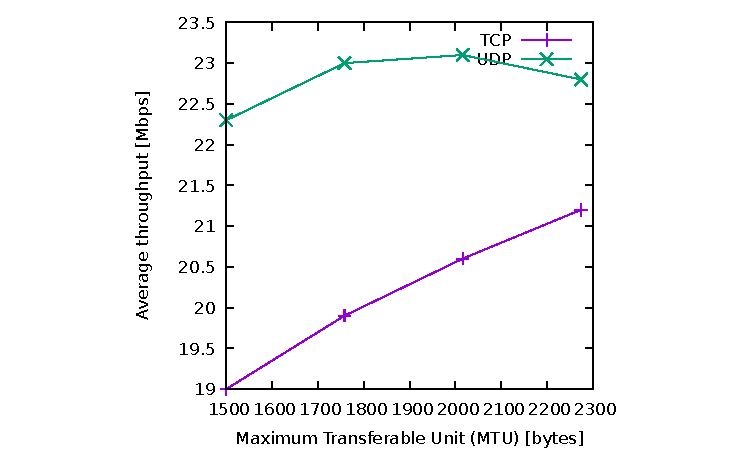
\includegraphics[width=0.5\textwidth]{traces/L3-4-1-tput.pdf} \\
UDP has a fairly small header per datagram. As overhead per datagram is already fairly limited, there is not much room for optimization by putting more data in each datagram. Additionally a larger datagram is more likely to get lost in a wireless network than a smaller one. We observe this when increasing the MTU from 2016 to 2274: the additional packet loss due to the larger frame size outweighs the decrease in per-bit overhead, leading to a lower throughput.
 \\ \\
In the case of TCP there is more per-bit overhead, meaning there is larger room for improvement by putting more data in each segment. Increasing the MTU consistently increases throughput for the tested range: additional packet loss never outweighs the performance increase of reducing the per-bit overhead. This is however never enough to overtake UDP performance.
